\chapter{Возможности протокола WebSocket}

\section{Основные принципы WebSocket}

Основные принципы WebSockets основаны на преодолении ограничений, существующих в протоколе HTTP.

\subsection{Двунаправленная связь}

Традиционный подход, основанный на протоколе HTTP, предполагает, что клиент инициирует запрос на сервер, а сервер отвечает на этот запрос. После ответа соединение закрывается. Это означает, что для каждой операции требуется инициировать новое соединение и отправить новый запрос, что может привести к значительным задержкам и накладным расходам на сеть. Кроме того, такой подход не применим для задач интерактивного взаимодействия между клиентом и сервером.

Протокол WebSocket позволяет установить постоянное двунаправленное соединение между сторонами. Двунаправленная связь означает возможность обмена данными в обоих направлениях - от клиента к серверу и от сервера к клиенту - без необходимости повторных запросов со стороны клиента. Технически, это означает что после первого запроса соединение между клиентом и сервером не завершается, а остается открытым в течение всей сессии. Таким образом обеспечивается возможность отправлять данные с сервера на клиент в любой момент без ожидания запроса от клиента. Клиент также может инициировать передачу данных серверу в режиме реального времени.

\subsection{Инициация соединения сервером}

В протоколе HTTP только клиент может инициировать соединение, отправляя запрос на сервер, а сервер может только отвечать на запросы (полудуплексное соединение). Это ограничение может быть проблематичным в ситуациях, когда серверу необходимо отправить данные клиенту без предварительного запроса от него. Сервер вынужден ожидать запроса от клиента, и только после этого отправить ответ.

Позволяя серверу инициировать передачу данных клиенту, WebSocket решает эту проблему. После установки постоянного соединения между клиентом и сервером с помощью протокола WebSocket, сервер может в любой момент отправлять данные клиенту без ожидания запроса. Это открывает возможности для мгновенного обновления информации на клиентской стороне. Такой подход может использоваться, к примеру, в системах мониторинга, когда нужно уведомить пользователя о наступлении какого-то события.

\subsection{Поддержка реального времени}

Протокол HTTP не поддерживает передачу в режиме реального времени, поскольку данные передаются только в ответ на запросы. Это затрудняет создание веб-приложений, которые требуют постоянного обновления данных в реальном времени. Чтобы клиент узнал об обновлении на сервере, ему приходилось реализовывать паттерн active waiting. Его суть сводится к тому, что клиентский код в бесконечном цикле отправляет запросы на сервер, ожидая получить обновления. Помимо избыточной нагрузки на обе стороны процесса, это порождало проблему оптимального выбора периодичности запросов: слишком частые запросы приводили с генерации мусорных пакетов в сети, а слишком редкие не позволяли достаточно оперативно забирать с сервера данные.

Благодаря WebSocket, сервер может отправить данные клиенту в момент их готовности, не ожидая запроса, обеспечивая поддержку реального времени в веб-приложениях что особенно полезно для чатов, многопользовательских игры, финансовых приложений и т. д.

\subsection{Эффективное использование ресурсов}

Основная оптимизация производительности, предоставляемая WebSocket, происходит из установлении постоянного соединения между клиентом и сервером. Повторяющиеся операции установления и завершения соединений являются довольно дорогой операцией. Особенно это чувствительно в мобильных устройствах, где есть повышенные требования к экономии ресурсов.

Следующей оптимизаций производительности является использование бинарных данных в заголовках. В традиционном HTTP все заголовки в текстовом формате ASCII и могут занимать ощутимую часть сетевого пакета. Переход к бинарным заголовкам позволяет снизить нагрузку на обработку данных и сократить объем передаваемой информации, что способствует общему ускорению работы системы.

Третья оптимизация производительности WebSocket заключается в поддерживает сжатие данных, что позволяет уменьшить размер передаваемых данных. Сервер и клиент могут договориться о методе сжатия, таком как \texttt{GZIP} или \texttt{DEFLATE}, и сжимать данные перед отправкой. Это помогает уменьшить объем данных, улучшая производительность и сокращая использование пропускной способности сети.

\subsection{Прокси-серверы и брандмауэры}

Прокси-сервера и брандмауэры играют важную роль в современных компьютерных сетях, поскольку способны обеспечить безопасность, контроль и масштабируемость, что особенно важно в корпоративных сетях. Однако использование этих технологий влечет ряд проблем для сетевого взаимодействия.

Одна из основных проблем, возникающих при из использовании, связана с поддержкой разных протоколов и стандартов. Отсутствие поддержки (или явно описанных правил) может вызывать конфликты и нежелательное поведение. Другой возможной проблемой может быть кеширование и буферизация данных. Традиционные соединения по своей природе обладают низким уровнем совместимости с прокси (к примеру, FTP), результатом чего является замедление передачи данных, а в худшем случае потеря или повреждение информации.

Протокол WebSocket разработан таким образом, что его работа осуществляется поверх протокола HTTP, что делает его совместимым с большинством прокси-серверов и фаерволов, избавляя пользователя от проблем с посредниками в коммуникации.

\section{Архитектура WebSocket}

\subsection{Установка и завершение соединения}

Протокол WebSocket предоставляет возможность установки двунаправленной связи между клиентом и сервером над одним устойчивым TCP-соединением. Большинство распространённых протоколов предполагают отправку первого пакета для рукопожатия на слушающий сокет сервера. Однако с WebSocket ситуация выглядит несколько сложнее, т.к. фактически отправляется стандартный HTTP запрос, но содержащий специальный заголовок.

В данном разделе мы пройдем через процесс установки и разрыва связи по WebSocket, а также рассмотрим суть и порядок отправления пакетов с каждой стороны.

Установка связи между клиентом и сервером начинается с выполнения HTTP-запроса с использованием метода "\texttt{GET}" и параметра "\texttt{Upgrade}". WebSocket использует этот параметр, чтобы сообщить серверу о своем желании переключиться на WebSocket-протокол.  

HTTP-запрос от клиента выглядит примерно так:

\begin{lstlisting}[style=CommandLineStyle]
GET /my-websocket-path HTTP/1.1
Host: server.example.com
Upgrade: websocket
Connection: Upgrade
Origin: http://example.com
Sec-WebSocket-Key: dGhlIHNhbXBsZSBub25jZQ==
Sec-WebSocket-Version: 13
\end{lstlisting}


Заголовок "\texttt{Sec-WebSocket-Key}" это уникальный ключ, который будет использоваться сервером для формирования ответа "\texttt{Sec-WebSocket-Accept}". Он нужен для того, чтобы сервер подтвердил, что он корректно обрабатывает именно WebSocket-запрос. Заголовок "\texttt{Sec-WebSocket-Version}" указывает версию протокола WebSocket. В этом примере используется версия 13, которая является наиболее актуальной на текущий момент.

После получения запроса сервер отправляет ответ (так же по HTTP), подтверждающий согласие на переход к WebSocket-протоколу. Ответ содержит "\texttt{101 Switching Protocols}" статус, "\texttt{Upgrade: websocket}" и "\texttt{Connection: Upgrade}" заголовки, а также "\texttt{Sec-WebSocket-Accept}", который создается на основе ключа "\texttt{Sec-WebSocket-Key}" из запроса клиента.

HTTP-ответ от сервера выглядит следующим образом:

\begin{lstlisting}[style=CommandLineStyle]
HTTP/1.1 101 Switching Protocols
Upgrade: websocket
Connection: Upgrade
Sec-WebSocket-Accept: dGhlIHNhbXBsZSBub25jZQ==
\end{lstlisting}

\subsubsection{Подпротоколы}

Помимо стандартного набора полей, существуют ещё подпротоколы (subprotocol), которые позволяют задать дополнительные заголовки \texttt{Sec-WebSocket-Extensions} и \texttt{Sec-WebSocket-Protocol} для управления потоком передачи.

Заголовок \texttt{Sec-WebSocket-Extensions: deflate-frame} указывает, что браузер поддерживает модификацию протокола, позволяющую сжимать данные. Обычно, этот заголок формируется браузером.

Заголовок \texttt{Sec-WebSocket-Protocol: soap, wamp} указывает, что браузер планирует передавать данные через WebSocket с использованием протоколов SOAP (Simple Object Access Protocol) или WAMP (WebSocket Application Messaging Protocol). Стандартные подпротоколы зарегистрированы в специальном каталоге IANA. При наличии таких заголовков сервер может использовать расширения и отправить соответствующий ответ.

Предположим, что в запросе клиент сообщил о поддержке сжатия, и готовности использовать протоколы SOAP и WAMP:

\fbox{
    \parbox{\textwidth}{%
    \texttt{\noindent
GET /my-websocket-path HTTP/1.1\\
Host: server.example.com\\
Upgrade: websocket\\
Connection: Upgrade\\
Origin: http://example.com\\
Sec-WebSocket-Key: dGhlIHNhbXBsZSBub25jZQ==\\
Sec-WebSocket-Version: 13\\
\hl{Sec-WebSocket-Extensions: deflate-frame\\
Sec-WebSocket-Protocol: soap, wamp}
    }}%
}

Сервер в ответе сообщил о поддержке расширения deflate-frame, но из запрошенных подпротоколов только SOAP:

\fbox{
    \parbox{\textwidth}{%
    \texttt{\noindent
HTTP/1.1 101 Switching Protocols\\
Upgrade: websocket\\
Connection: Upgrade\\
Sec-WebSocket-Accept: dGhlIHNhbXBsZSBub25jZQ==\\
\hl{Sec-WebSocket-Extensions: deflate-frame\\
Sec-WebSocket-Protocol: soap}
    }}%
}

После успешного переключения на протокол WebSocket между клиентом и сервером становится доступным двунаправленный обмен данными через набор WebSocket-фреймов (или сообщений). Фреймы можно отправлять в любых допустимых форматах:
\begin{enumerate}
\item кадры, которые передают текстовую информацию представленную в кодировке utf-8;
\item кадры, которые передают данные в двоичном виде;
\item кадры, которые содержат управляющие команды (ping, pong, close).
\end{enumerate}
Одна из сторон может инициировать разрыв соединения, отправляя управляющий фрейм "close" с опциональным статус кодом и причиной закрытия.

\subsubsection{Завершение соединения}

Процесс разрыва связи между клиентом и сервером следующий:

\begin{enumerate}
\item Одна из сторон (клиент или сервер) отправляет управляющий фрейм "close" с определенным статусом и возможным сообщением о закрытии;
\item Принимающая сторона подтверждает получение фрейма "close", отправляя свой фрейм "close" с любым желаемым статусом и сообщением;
\item После успешного обмена управляющими фреймами "close" TCP-соединение закрывается;
\item Каждая из сторон выполняет нужные действия по уведомлению об отключении, очистке ресурсов и прочему.
\end{enumerate}

Вебсокеты используют четырехзначные коды закрытия (event code), которые отличаются от HTTP-кодов:
\begin{itemize}
\item 1000: Соединение закрыто нормальным образом.
\item 1001: Противоположная сторона "пропала". Это может произойти, когда серверный процесс был завершен или браузер перешел на другую страницу.
\item 1002: Соединение закрыто противоположной стороной из-за ошибки в протоколе.
\item 1003: Соединение закрыто, потому что противоположная сторона не может принять полученные данные. Например, если сторона, которая работает только с текстовыми данными, получает бинарное сообщение, она может закрыть соединение с данным кодом.
\end{itemize}

Таким образом, протокол WebSocket обеспечивает поддержку установки и разрыва связи между клиентом и сервером через процесс обмена HTTP-запросами и ответами, а затем переключением на двунаправленный обмен данными. Отправка пакетов (фреймов) между сторонами происходит согласно спецификации WebSocket, которая определяет формат и последовательность отправляемой информации и управляющих команд.

\subsection{Фреймы и их структура}

Формат пакета WebSocket был разработан для минимизации сложности парсинга и накладных расходов, связанных с обменом данных. Все фреймы можно разделить на две категории: data frames (фреймы с данными) и control frames (фреймы управления). Первые предназначены для передачи полезной нагрузки, а вторые обеспечивают задачи поддержки связи (PING) и закрытия соединения.

На рисунке 1.1 приведена схема фрейма из RFC6455 раздел 5.2 \cite{label2}.

Пакет состоит из заголовка и полезной нагрузки. Заголовок пакета имеет длину от 2 до 14 октетов, в зависимости от модификаторов в полях заголовка. Начинатается заголовок пакета с поля \texttt{FIN} (вертикальная надпись на рисунке), затем поля \texttt{RSV1}, \texttt{RSV2}, \texttt{RSV3}. Все они занимают всего один бит. После идёт поле \texttt{oppcode} (4 бита), \texttt{MASK} (1 бит) и дальше \texttt{Payload len} (7 бит), которое показывает размер "длинны тела" пакета. Затем, если "длинна тела" равна 126 или 127, идёт "расширенная длина тела", и потом (на следующей строке, то есть после первых 32 бит) будет её продолжение. После идёт ключ маски и дальше сами данные.

\begin{figure}[H]
\centering
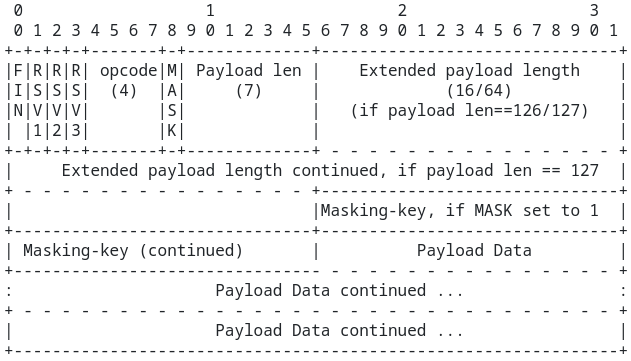
\includegraphics[scale=0.8]{res/ws-frame}
\caption{Фрейм WebSocket протокола}
\end{figure}


Теперь подробнее рассмотрим назначение флагов и возможные значения:
\begin{itemize}
\item \texttt{FIN} -- это 1-битовый флаг, указывающий, является ли обрабатываемый пакет последним фрагментом в сообщении. Значение 0 означает промежуточный пакет, а 1 -- последний пакет. Таким образом, если передаётся длинное сообщение, то 1 будет только у последнего пакета, а если короктое -- то у одного единственного (первого и последнего) пакета.
\item \texttt{RSV (Reserved bits)} -- это 3 битовых флага, отведенный для будущих расширений протокола. RSV1, RSV2 и RSV3 должны иметь значение 0, если они не используются каким-либо расширением.
\item \texttt{OpCode} --это 4-битовый код, определяющий вид полезной нагрузки. Значение OpCode может быть:
\begin{itemize}
	\item \texttt{0x1} обозначает текстовый фрейм.
    \item \texttt{0x2} обозначает двоичный фрейм.
    \item \texttt{0x3} зарезервированы для будущих фреймов с данными.
    \item \texttt{0x4} зарезервированы для будущих фреймов с данными.
    \item \texttt{0x5} зарезервированы для будущих фреймов с данными.
    \item \texttt{0x6} зарезервированы для будущих фреймов с данными.
    \item \texttt{0x7} зарезервированы для будущих фреймов с данными.
    \item \texttt{0x8} обозначает закрытие соединения этим фреймом.
    \item \texttt{0x9} обозначает PING.
    \item \texttt{0xA} обозначает PONG.
    \item \texttt{0xB} зарезервированы для будущих управляющих фреймов.
    \item \texttt{0xC} зарезервированы для будущих управляющих фреймов.
    \item \texttt{0xD} зарезервированы для будущих управляющих фреймов.
    \item \texttt{0xE} зарезервированы для будущих управляющих фреймов.
    \item \texttt{0xF} зарезервированы для будущих управляющих фреймов.
    \item \texttt{0x0} обозначает фрейм-продолжение для фрагментированного сообщения. Он интерпретируется, исходя из ближайшего предыдущего ненулевого типа.
\end{itemize}
\item \texttt{MASK} -- это 1-битовый флаг, указывающий, применяется ли маска к полезной нагрузке. Для всех отправляемых клиентом сообщений \texttt{MASK} должен быть равен 1, а для всех сообщений сервера — равен 0.
\item \texttt{Payload len} -- это поле может занимать 7 битов, 7+16 битов, или 7+64 битов и хранит длинну тела, т.е. размер передаваемых данных.
\begin{itemize}
    \item "0-125" указывает длину полезной нагрузки в октетах;
    \item "126" указывает, что следующие 2 октета интерпретируются как 16-битное беззнаковое целое число, определяющее длину полезной нагрузки;
    \item "127" указывает, что следующие 8 октетов интерпретируются как 64-битное беззнаковое целое число, определяющее длину полезной нагрузки.
\end{itemize}
Эта сложная схема необходима для минимизации издержек: рассмотрим сообщений длиной 125 байт (и менее), тогда для хранения длины потребует всего 7 битов; для больших сообщений (в пределах 65536) -- 7 битов + 2 байта; а для еще ещё больших -- 7 битов и 8 байт. Этого будет достаточно для хранения длины сообщения размером в гигабайт и более.
\item \texttt{Masking-key} -- если флаг \texttt{MASK} установлено 0, то этого полня нет; иначе, это 4-байтное поле содержат маску, которая налагается на тело сообщения.
\item \texttt{Payloat data} -- После заголовка следует полезная нагрузка, которая может включать текстовые или двоичные данные. Маскировка предотвращает возникновение проблем на уровне более низких слоев сетевой инфраструктуры, связанных с неконтролируемым форматом бинарных данных.
\end{itemize}

\subsubsection{Примеры пакетов}

Не фрагментированное текстовое сообщение "Hello" без маски может выглядеть так:

\begin{lstlisting}[style=CommandLineStyle]
0x81 0x05 0x48 0x65 0x6c 0x6c 0x6f
\end{lstlisting}

Состояние флагов будет следующим:
\begin{itemize}
\item \texttt{FIN = 1} -- это короткое сообщение, первый пакет является и последним;
\item \texttt{OpCode = 0x1} -- простой текстовый фрейм.
\end{itemize}

Таким образом, мы получаем \texttt{10000001} в двоичной системе счисления, или \texttt{0x81} в шестнадцатеричной. Полосе заголовка идёт размер длинны тела (\texttt{0x5}) и само тело с текстом.

Фрагментированное текстовое сообщение "Hello", " ", "World" (из трёх частей), без маски может выглядеть так:
\begin{lstlisting}[style=CommandLineStyle]
0x01 0x05 0x48 0x65 0x6c 0x6c 0x6f
0x00 0x01 0x20
0x80 0x05 0x57 0x6f 0x72 0x6c 0x64
\end{lstlisting}

Состояние флагов будет следующим:
\begin{itemize}
\item У первого фрейма \texttt{FIN = 0} и текстовый опкод \texttt{OpCode = 0x1};
\item у второго фрейма \texttt{FIN = 0} и \texttt{OpCode = 0x0} (при фрагментации сообщения, у всех фреймов, кроме первого, опкод пустой);
\item У третьего (завершающего) фрейма \texttt{FIN = 1}.
\end{itemize}

\subsection{WebSocket API}

WebSocket объект обеспечивает API для установки и контроля веб-сокет соединения с сервером, а также для передачи и приема данных через данное соединение. На данный момент полная спецификация поддерживается всеми браузерами \cite{label3}.

Конструктор WebSocket имеет один обязательный параметр и один необязательный параметр:

\begin{lstlisting}[style=CommandLineStyle]
WebSocket WebSocket(
  in DOMString url,
  in optional DOMString protocols
);

WebSocket WebSocket(
  in DOMString url,
  in optional DOMString[] protocols
);
\end{lstlisting}

\begin{itemize}
\item \texttt{url} -- ссылка для подключения; сервер по данному адресу должен откликнуться на запрос websocket.
\item \texttt{protocols} (опционально) -- протокол представлен в виде строки или списка строк протоколов. Эти строки служат для определения клиентских подпротоколов, поскольку один сервер может поддерживать различные WebSocket-подпротоколы (например, чтобы один сервер мог обрабатывать разные виды коммуникаций на основе указанного протокола). Если значение протокола не указано, по умолчанию используется пустая строка.
\end{itemize}

Если порт, на который устанавливается соединение заблокирован, конструктор может выбросить исключение "\texttt{SECURITY\_ERR}".

\subsubsection{Константы состояния готовности}

Константы используются атрибутом \texttt{readyState} для описания состояния WebSocket подключения

\begin{itemize}
\item \texttt{CONNECTING} -- Соединение ещё не открыто.
\item \texttt{OPEN} -- Соединение открыто и готово к обмену данными.
\item \texttt{CLOSING} -- Соединение в процессе закрытия.
\item \texttt{CLOSED} -- Соединение закрыто или не может открыться.
\end{itemize}

\subsubsection{Методы}

\texttt{close()}. Закрывает WebSocket - подключение или заканчивает попытку подключения. Если подключение уже закрыто, этот метод не делает ничего.

\texttt{send()}. Передаёт данные на сервер через WebSocket - соединение.

\section{Сравнение WebSocket с другими технологиями}

\subsection{HTTP-поллинг}


Длинные опросы (long polling) -- это технология, которая была разработана для решения проблемы латентности при использовании обычных опросов (веб-запросов с задержками), вызванных ограничениями стандартных HTTP-соединений. Вместо того чтобы постоянно отправлять новые запросы на сервер для проверки обновлений и тем самым создавать большую нагрузку на сервер, длинный опрос позволяет клиенту отправить один запрос, который будет "держаться" сервером, пока не появится новая информация для отправки клиенту. После отправки этой новой информации сервер закрывает соединение, и клиент немедленно запрашивает новое подключение.

Главным преимуществом длинных опросов является его совместимость с большинством существующих веб-серверов и HTTP-инфраструктуры, что упрощает его интеграцию в уже развернутые системы. Однако, длинные опросы могут столкнуться с ограничениями производительности из-за потребности в постоянной отправке новых запросов и создания новых подключений, что может вызвать задержку при передаче данных. Особенно это заметно при большом количестве активных клиентов.

В то же время, WebSocket обеспечивает более высокую производительность, так как постоянное соединение устраняет задержку и снижает расходы на обработку запросов. Кроме того, WebSocket обеспечивают лучшую поддержку двоичных данных и сжатия, что позволяет сократить объем передаваемых данных и ускорить их обмен. Недостатки WebSocket связанные с поддержкой браузерами уже в прошлом.

В зависимости от конкретного проекта и требований, можно использовать как длинные опросы, так и WebSocket. Если важно сохранение совместимости с существующими клиентами (к примеру, устаревшие версии Android) и инфраструктурой, и потребность в активной связи между клиентом и сервером не является критичной, то можно использовать длинные опросы. Однако, если проект требует быстрой и эффективной передачи данных с минимальными задержками, WebSocket является более оптимальным выбором для реализации взаимодействия между клиентом и сервером.

\subsection{Server-Sent Events (SSE)}

Server-Sent Events (SSE) представляет собой технологию, позволяющую серверу отправлять обновления клиенту через односторонний HTTP-канал без необходимости инициирования новых запросов со стороны клиента. SSE обычно используется для отправки уведомлений или обновлений статуса устройств, что в свою очередь позволяет снизить нагрузку на сервер и повысить скорость обмена данными.

Основное отличие между Server-Sent Events (SSE) и WebSocket состоит в режиме коммуникации. SSE предоставляет только одностороннее подключение (от сервера к клиенту), в то время как WebSocket обеспечивает двустороннее общение. Это означает, что SSE идеально подходит для ситуаций, где серверу необходимо отправлять информацию клиенту, но клиент не обязан отсылать данные серверу. Однако, если клиенту требуется отправить данные серверу, например, для обработки пользовательского ввода, WebSocket будет предпочтительнее.

С точки зрения производительности и надежности, Server-Sent Events и WebSocket можно считать сравнительно равными. Обе технологии обладают низкими задержками и малым оверхедом, что делает их подходящими для использования в интерактивных приложениях. Однако стоит обратить внимание на то, что некоторые функции, доступные в WebSocket, отсутствуют в SSE. К таким функциям относится, например, возможность отправки бинарных данных.

Выбор между Server-Sent Events и WebSocket зависит от конкретных задач, которые ставятся перед разработчиками. SSE подходит для ситуаций с однонаправленным обменом данными, особенно если серверу необходимо отправлять частые обновления клиенту. WebSocket же является идеальным решением для двусторонних взаимодействий и приложений, где важна реакция на пользовательский ввод в режиме реального времени.

\subsection{WebRTC}

Технология WebRTC (Web Real-Time Communications) была разработана для обмена данными в режиме реального времени между двумя браузерами без участия централизованного сервера. Она поддерживает передачу потоковых данных, таких как аудио, видео и единственные наборы данных бинарных и обычных текстовых форм. WebRTC состоит из трех основных API: MediaStream, RTCPeerConnection и RTCDataChannel. Эти API работают совместно, чтобы установить пару pub/sub (поведенческий шаблон проектирования передачи сообщений "Издатель - подписчик") с использованием протоколов SCTP и ICE (включая STUN и TURN). Ключевым аспектом WebRTC является возможность значительно снижать задержку обмена данными и работать в условиях реального времени. Это делает технологию WebRTC чрезвычайно полезной для видео- и аудиоконференций, P2P-игры и других решений, требующих быстрого взаимодействия между участниками.

WebSocket, с другой стороны, представляет собой универсальный протокол для обмена данными между клиентом и сервером, построенный поверх протокола HTTP, который поддерживает инициацию соединения на сервере. WebSocket работает через TCP, что может привести к задержкам из-за перегрузки сети или медленной передачи данных. В отличие от WebRTC, WebSocket требует промежуточного сервера для обработки запросов от клиента, что увеличивает задержки и зависимость от сервера.

Сравнивая технические характеристики, можно отметить, что WebRTC имеет больше возможностей, включая адаптивное кодирование, снижение задержки и аппаратные возможности ускорения через GPU. WebSocket имеет более простую структуру, что облегчает развертывание и снижает нагрузку на сервер. Однако необходимость использования серверов делает WebSocket более затратной технологией по сравнению с децентрализованным подходом WebRTC.

В итоге можно сказать, что WebRTC и WebSocket представляют разные классы технологий, каждая из которых имеет свои достоинства и недостатки. WebRTC подходит для видеочатов, тогда как WebSocket решает проблему обмена сообщениями. В некоторых ситуациях возможно использование обеих технологий в одной системе, с учетом уникальных преимуществ каждой из них.